\documentclass[12pt,a4paper]{article}
\usepackage{amsfonts, amssymb, amsmath}
\usepackage{fullpage}
\usepackage{parskip} % skip a line instead of indenting
\usepackage{graphicx} % for inserting images
\usepackage{amsthm}
\usepackage{xcolor}
\usepackage{tikz} % for plot

\title{Algorithms}
\author{R4 Cheng}
\date{\today}

\newcommand{\remark}[1]{
    {\small $>$ {\color{blue} #1}}
}

\begin{document}
\maketitle

\textbf{Def.} Introduction of precise, umambiguous, and correct procedures for solving general problems

We care how many clicks in debug mode

\section*{Runtime Analysis}

Runtime is expressed by counting the number of steps, as funtion of \textbf{the size of the input}

Asymptotic Notations:

\begin{itemize}
  \item Big $O$: upper bound on the growth rate
  \item Little $o$: "strict" upper bound on the growth rate
  \item Big $\Omega$: lower bound on the growth rate
  \item $\Theta$: tight bound on the growth rate
\end{itemize}

$f(n)$: the runtime of an algorithm for input size $n$

$g(n)$: a simplified function without constants, lower order terms, e.g. $n^2$, $n \log n$

\textbf{Big-O Definition}: It is said $f(n) = O(g(n)) \iff$ there exists a constant $c > 0$ and $n_0 > 0$ such that

\[f(n) \leq c \cdot g(n) \text{ for all } n \geq n_0\]

\textbf{Little-o Definition}:

\[f(n) = o(g(n)) \iff \lim_{n \to \infty} \frac{f(n)}{g(n)} = 0\]

E.g. $f(n) = 3900n + 57800$

$f(n) = o(n^2)$? T, because $\lim_{n \to \infty} \frac{3900n + 57800}{n^2} = 0$

$f(n) = o(n)$? F, because $\lim_{n \to \infty} \frac{3900n + 57800}{n} = 3900$

\textbf{Big-$\Omega$ Definition}: It is said $f(n) = \Omega(g(n)) \iff$ there exists a constant $c > 0$ and $n_0 > 0$ such that
$$f(n) \geq c \cdot g(n) \text{ for all } n \geq n_0$$

\subsection*{Relation between $O,o,\Omega,\theta$}

\begin{itemize}
    \item $f = \theta(g) \iff f = O(g),f = \Omega(g)$
    \item $f = o(g) \Rightarrow f = O(g)$
    \item $f = O(g) \iff g = \Omega(f)$
    \item $f = \theta(g) \iff g = O(f)$
\end{itemize}

\textbf{Caveats about constants}

For $\log_4(n)$, is 4 ignorable? No, it matters

\remark{$log_a(x) = log_a blog_b(x)$}

\includegraphics[width=\textwidth]{./images/common_efficiency_class.png}

\section*{Merge Sort}

\[T(n) = 2T(\frac{n}{2}) + 2n + c\]

\remark{$2n$: compare and copy n elements $= 2n$}

\textbf{Proof}

\[T(n) = 2T(\frac{n}{2}) + 2n + c\]
\[\Rightarrow T(\frac{n}{2}) = 2T(\frac{n}{4}) + (n + c)\]
\[\Rightarrow T(\frac{n}{4}) = 2T(\frac{n}{8}) + (\frac{n}{2} + c)\] Bring in $T(\frac{n}{2})$
\[\Rightarrow T(n) = 2\{2T(\frac{n}{4}) + (n + c)\} + 2n + c\]
\[= 2^2T(\frac{n}{2^2}) + 2 \cdot 2n + c + 2c\] Bring in $T(\frac{n}{4})$
\[= 2^2\{2T(\frac{n}{8}) + (\frac{n}{2} + c)\} + 2 \cdot 2n + c + 2c\]
\[= 2^3T(\frac{n}{2^3}) + 3 \cdot 2n + c + 2c + 4c\]
\[\Rightarrow T(n)= 2^kT(\frac{n}{2^k}) + k \cdot 2n + (2^k-1)c\]

Since $T(1) = 1$, $\frac{n}{2^k} = 1 \Rightarrow k = \log_2(n)$

\[\Rightarrow T(n) = n \cdot 1 + \log_2(n) \cdot 2n + (n-1)c\]
\[\Rightarrow T(n) = O(nlogn) \]

\section*{Master Theorem}

\[T(n) = aT(\frac{n}{b}) + cn^d\]
\[\Rightarrow T(n) = (1 + \frac{a}{b^d}^2 + \cdots + \frac{a}{b^d}^k)cn^d\]

$a$: number of subproblems

$b$: factor by which the problem size is reduced

$d$: exponent in the running time of the "combine" step

\textbf{Case 1}: $a < b^d$, or equiv. $d > log_ba, T(n) = O(n^d)$
$\Rightarrow$ the cost of the "combine" step dominates the cost of the "split" step

\textbf{Case 2}: $a = b^d$, or equiv. $d = log_ba, T(n) = O(n^d \log n)$

\textbf{Case 3}: $a > b^d$, or equiv. $d < log_ba, T(n) = O(n^{log_ba})$

\section*{Proof by induction}

\remark{Useful for proving correctness of recursive algorithms}

\section*{Devide and Conquer}

\subsection*{Inversion Counting}

Input: an A comtaining numbers $1,2,\dots,n$ in some arbitrary order

Output: the number of inversions in $A$, i.e. the number of pairs $(i,j)$ of array indices with $i < j$ and $A[i] > A[j]$

It is useful for recommender systems $\Rightarrow$ fewer inversions means better alignment with user preferences.



\subsection*{Quick Select}

Worst case: $ T(n) = T(n-1) + cn \Rightarrow O(n^2)$

Best case: $ T(n) = T(n/2) + cn \Rightarrow O(n)$

\subsection*{Median}

Input: A list of numbers $S$; an integer $k$

Output: the $k$th smallest element of $S$

\subsubsection{A randomized divide-and-conquer algorithm}

\[S_k = \]

\subsubsection*{Smart Selection of Pivot}

Break array $A$ into chunks of fives and find the median of each chunk,
constructing a new array $M$ of medians.

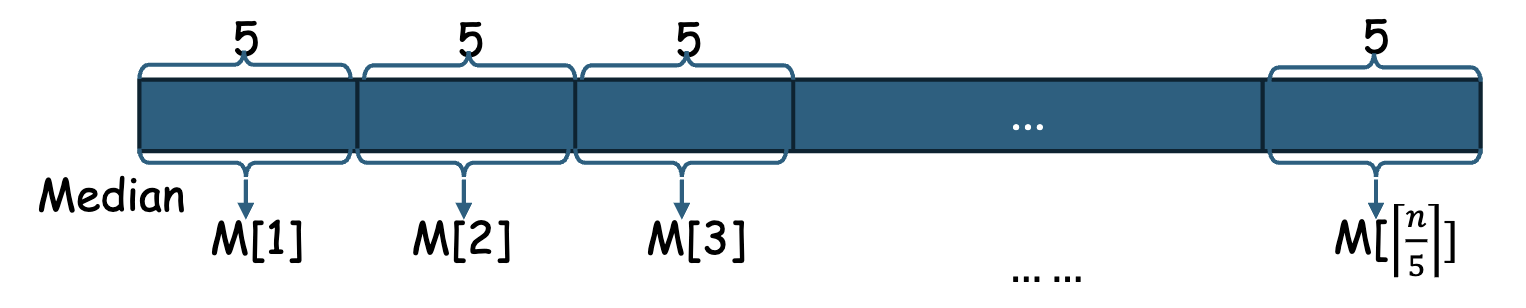
\includegraphics[width=\textwidth]{./images/chunks_of_fives.png}

And \textbf{median} of $M$ aka. $MM$ is the pivot.

\textbf{Claim:} $MM$ is at least $\geq \frac{3}{10}A$ and $\leq \frac{3}{10}A$

\textbf{Proof:} $MM$ is the median of medians, so $\frac{1}{2}$ medians in $M$ are $\leq MM$.
$\because M = \frac{A}{5} \Rightarrow \frac{A}{10}$ medians are $\leq MM$. Moreover, 
For each $M[i]$, there are 3 elements $\leq M[i]$ $\therefore \frac{3A}{10} \leq MM$

\begin{verbatim}
Select(A, k)
1. for i = 1, ..., n/5
2.     M[i] = median (a[5(i-1)+1], 5i)
3. MM = Select(M, n/10)
4. v = index of MM in A
5. r = partition(A, v)
6. if k=r: return A[r]
7. if k<r: Select(A[1,...,r-1], k)
8. if k>r: Select(A[r+1,...,n], k-r)
\end{verbatim}

\[T(n) \leq O(n) + T(n/5) + T(7n/10) \Rightarrow T(n) = O(n)\]

\section*{Dynamic Programming}

The main question in dynamic programming always is, what are the subproblems?

\subsection*{Fibonacci}

\[T(n) = T(n-1) + T(n-2) + c\]
\[\Rightarrow T(n) \leq 2T(n-1) + c\]
\[\Rightarrow T(n) \leq 2^2T(n-2) + 2c + c\]
\[\Rightarrow T(n) \leq 2^kT(n-k) + kc\]
\[k = n - 1 \Rightarrow T(n) \leq O(2^n)\]

\[T(n) \geq 2T(n-2) + c = \Omega(2^{\frac{n}{2}})\]



\subsection*{Applications of DP}

\begin{itemize}
  \item Unix diff for comparing files
  \item Bellman-Ford for shortest path
  \item CKY algorithm for natural language parsing
  \item etc.
\end{itemize}

\subsection*{Longest Increasing Subsequence}

\[L(i) = \text{the length of a longest increasing subsequence ending at position i}\]
\[L(i) = (\max_{j:a_j < a_i}{L(j)})+1\]

\subsection*{Edit Distance}

\[D(i, j) = \text{the edit distance between} s_1,s_2,\dots,s_i \text{and} t_1,t_2,\dots,t_j\]

\subsection*{Maximum Subarray}

Because the decision at each index depends only on the previous index,
it is uncessary to define $L(i, j) = $ the maximum subarray sum from index $i$ to $j$.
Instead, we can define $L(i) = $ the maximum subarray sum ending at index $i$.

\subsection*{Knapsack}

\remark{If the input is very sparse so that very few subproblems are solved, then top-down is a lot faster; if the input is very dense so that most subproblems are solved, then bottom-up is slightly faster (due to avoiding the overhead for recursion).}

Q: For max $W$ pounds, there are $n$ items to pick from, of weight $w_1, \dots, w_n$ and dollar value $v_1, \dot, v_n$. 
What is the most valuable combination of items he can fit into his bag?

E.g., take $W = 10$ and 

\begin{table}[h]
    \centering
    \begin{tabular}{c c r}
        \textbf{Item} & \textbf{Weight} & \textbf{Value} \\
        1 & 6 & \$30 \\
        2 & 3 & \$14 \\
        3 & 4 & \$16 \\
        4 & 2 & \$9 \\
    \end{tabular}
\end{table}

\subsubsection*{0-1 knapsack problem}

\remark{go to local convenience store}

\remark{aka. the subset sum problem}

Intuition: Go greedy

\begin{enumerate}
  \item Greedily choose the most valuable item?
  \item Greedily choose the most value/weight item?
\end{enumerate}

Sadly, both can be found a counter example.

$K(w, j) =$ maximum value achievable using a knapsack of capacity $w$ and items $1, 2, \dots, j$

We should consider both capacity $w$ and items $j$, where $0 \leq j \leq n$

$\Rightarrow$

The answer we seek is $K(W, n)$

Subproblems:

1. Choose the current item: $K(w - w_j, j - 1) + v_j$ \\
2. Don't choose the current item: $K(w, j - 1)$

\[
\Rightarrow
K(w, j) = \max \left\{
\begin{array}{l}
    K(w - w_j, j - 1) + v_j \\
    K(w, j - 1)
\end{array}
\right.
\]

\begin{center}
(The first case is invoked only if $w_j \leq w$)
\end{center}

\remark{we can express $K(w, j)$ in terms of subproblems $K(\cdot, j - 1)$.}

Time complexity: $O(nW)$

\subsubsection*{Unbounded knapsack problem}

\remark{aka. Knapsack with repetition}

\remark{like go to Costco (unlimited supply)}

\[K(w) = \text{maximum value achievable with a knapsack of capacity } w\]

Express this in terms of smaller subproblems:

\[
K(w) = \max_{i : w_i \leq w} \{ K(w - w_i) + v_i \},
\]

\begin{verbatim}
    K(0) = 0
    for w = 1 to W:
        K(w) = max {K(w - w_i) + vi: w_i <= w}
    return K(W)
\end{verbatim}

It is 1D dynamic programming. Each entry can take up to $O(n)$ time to compute, so the overall runtime is $O(nW)$ 

\subsection*{Optimal binary search tree}

Q: what is the time complexity for this q?

TODO: study Longest common subsequence

\subsection*{Longest Common Subsequence}

\section*{Greedy Algorithms}

Greedy template:
\begin{verbatim}
Let T be the set of tasks H is the rule determinging the greedy algorithm

A = {}
While (T is not empty)
    Select a task t from T by a rule H
    Add t to A
    Remove t and all tasks imcompatible with t from T
\end{verbatim}

\subsection*{Proving the optimality of a greedy algorithm}

\subsubsection*{Greedy stays ahead}

\subsubsection*{Exchange argument}

\subsection*{Scheduling Theory}

\subsubsection{Interval Scheduling}

\begin{verbatim}
    f()
\end{verbatim}

Prove:

the \textbf{Earlist-Finish-Time} algorithm is optimal.

We need to show that the solution chosen by greedy is as good as any other solution.

Usually, use the strategy of proof by contradiction

\subsection*{Minimum Spanning Tree}

\remark{aka. every node should be connected to every other node}

We assume the graph is undirected in this class.

\subsubsection{Applications of MST}

\begin{itemize}
    \item Network design
    \item Approximations to NP-hard problems like traveling salesman problem
    \item Clustering in machine learning
\end{itemize}

\subsubsection{Greedy Template for MST}

\begin{verbatim}
Init an empty set of edges T
While T is not yet a spanning tree (|T| <= |V| - 1) 
    select $e \in E$ to add to $T$ according to a greedy criterion
Return T
\end{verbatim}

Kruskal's Algorithm: sort edges by weight, add edge to $T$ if it doesn't create a cycle

Prim's Algorithm: start at any node, add the lightest edge to $T$ that connects a node in $T$ to a node not in $T$

\subsubsection{Proof of Correctness}

Use \textbf{cut property}: If we can partition the graph into two parts, 
and an edge $e$ is the cheapest edge connecting across the two parts, then $e$ must be in the MST.

\subsection*{Huffman coding}

Claim: The optimal code must be a full binary tree

\begin{verbatim}
// C: the set of tokens, f: the frequency of each token
Huffman_recur(C, f)
    Identify the two least frequent tokens x, y in C
    C' = C - {x, y} + {z} // z = x + y
    Assign frequency for z: f(z) = f(x) + f(y)
    T' = Huffman_recur(C', f)
    Append x and y as children of z in T'
    return T'
\end{verbatim}

\subsubsection*{Proof Greedy Choice Property}

Let $x,y$ be the two least frequent tokens of $C$.
There exists an optimal tree in which $x$ and $y$ are siblings.

\(\Rightarrow\) use \textbf{the exchange argument}

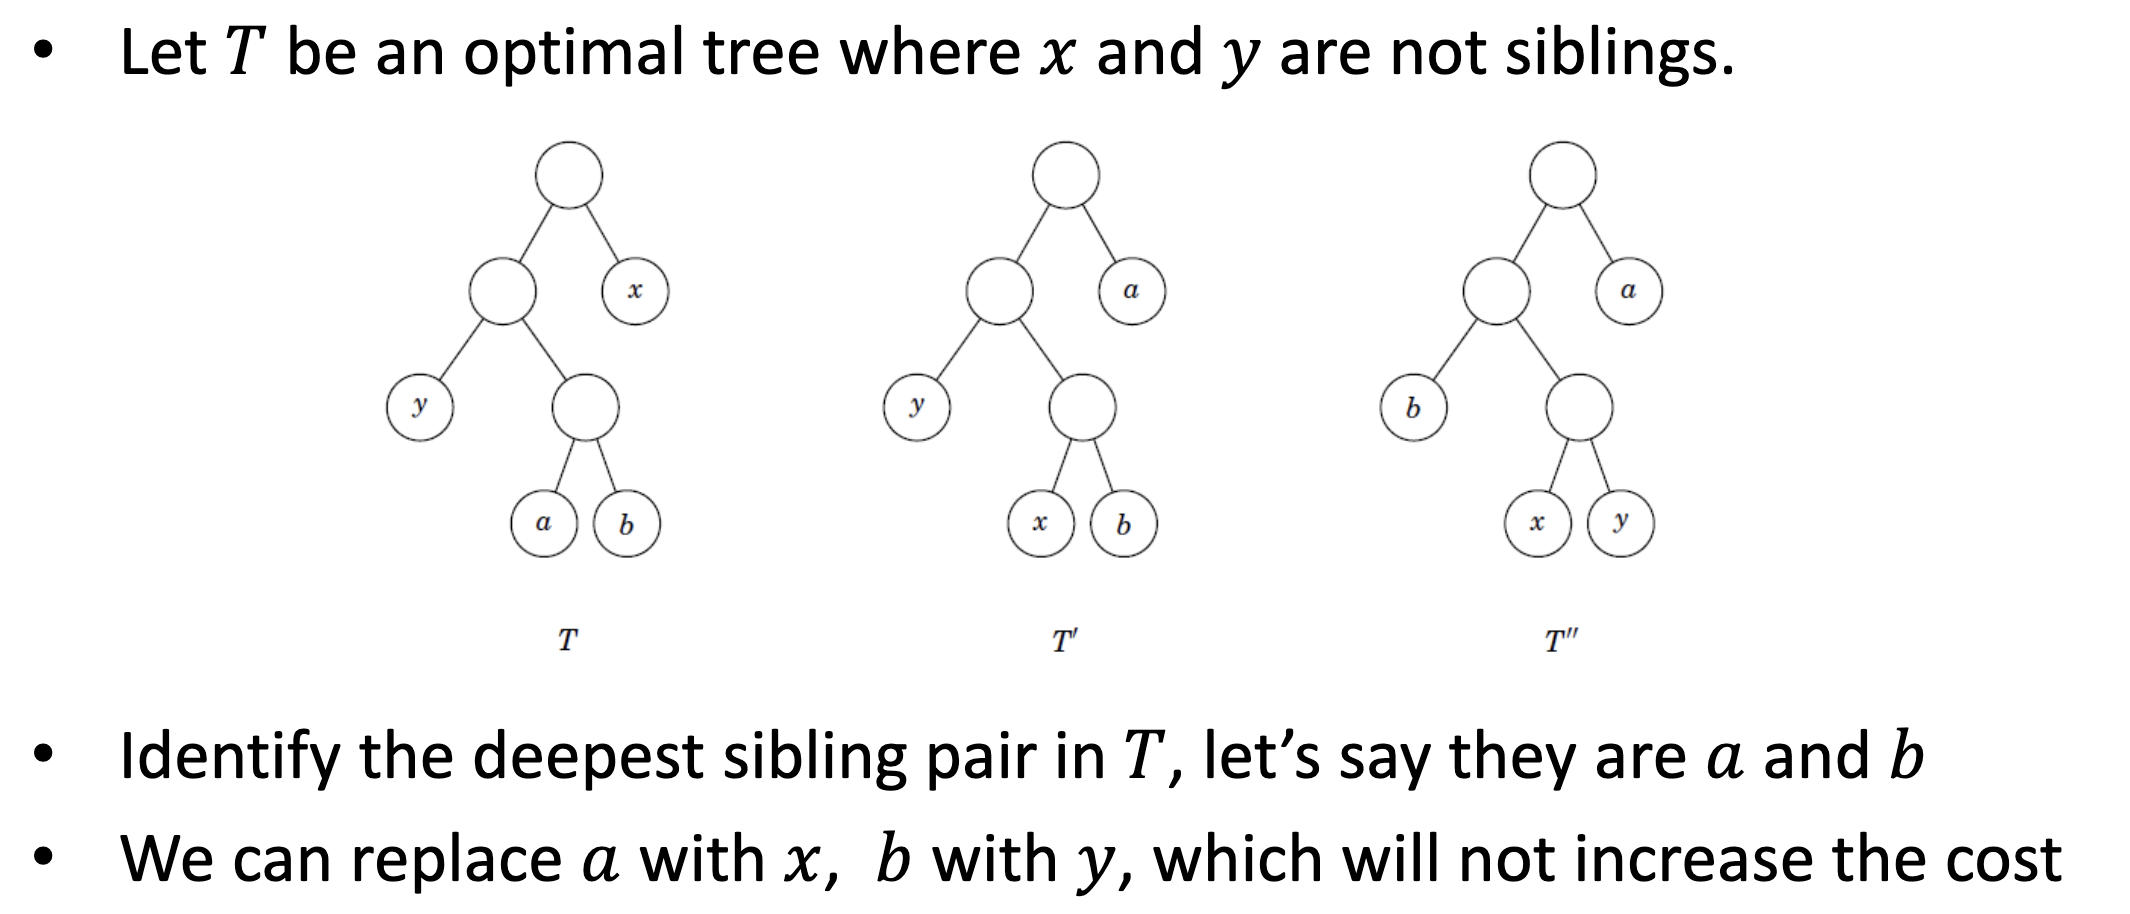
\includegraphics[width=\textwidth]{./images/the_exchange_argument.png}

\subsubsection*{Proof Corrrectness of Huffman's Algorithm}

\textbf{Proof by induction:}

Base case: $n=2$ and 1 bit for each token

Inductive hypothesis: 

Assume that the algorithm produce an optimal code for all token of $2,\dots,k$

Inductive step:

\section*{Graph}

Sparse vs. Dense

\begin{itemize}
    \item Sparse: $|E| = \text{degree} \cdot |V| = O(|V|)$
    \begin{itemize}
        \item The world is sparsely connected but well connected, which is known as the ``small world phenomenon". 
    \end{itemize}
    \item Dense: $|E| = O(|V|^2)$
    \begin{itemize}
        \item very small, e.g., family, single round robin tournament
    \end{itemize}
\end{itemize}

\subsection*{Directed acyclic graph (DAG)}

\begin{itemize}
    \item E.g., software dependency, course prerequisite
    \item Each DAG has at least one \textbf{topological order}.
\end{itemize}

\begin{figure}[h]
    \centering
    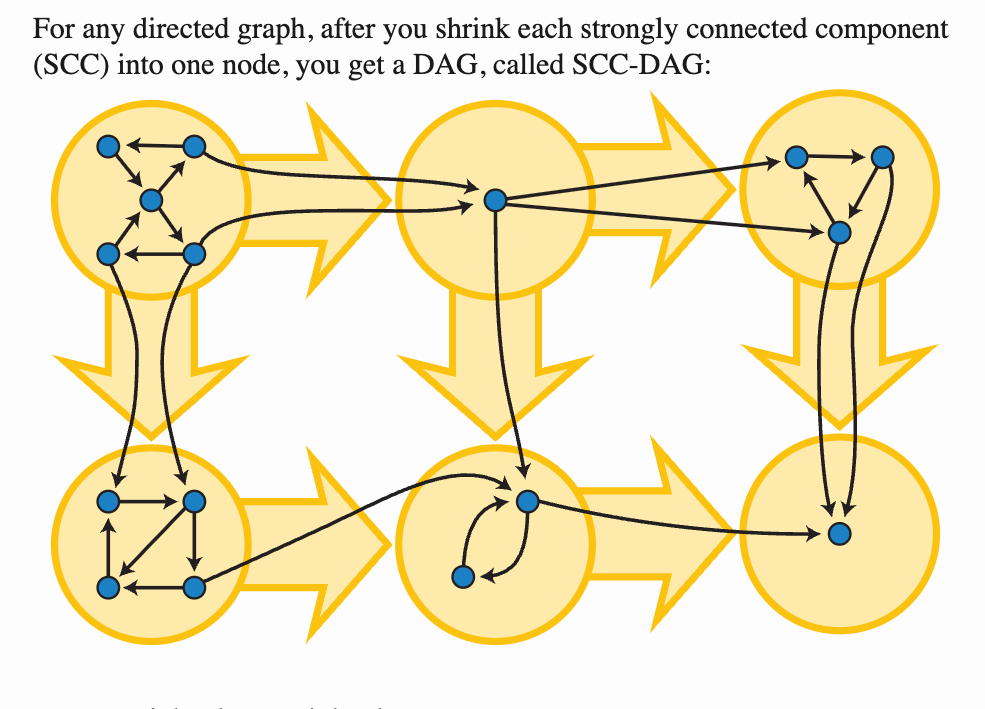
\includegraphics[width=\textwidth]{./images/scc_dag.png}
    \caption{SCC DAG}
    \label{fig:scc_dag}
\end{figure}

\subsection{Representations}

Adjacency Matrix:

We use a $|V| \times |V|$ matrix $A$ to represent the graph $G = (V, E)$,
where each $A_{i,j} = 1 \text{ or } c(i, j)$

Notes that:

\begin{itemize}
    \item the matrix is symmetric for undirected graphs and asymmetric for directed graphs.
    \item the matrix Representation, using $O(|V|^2)$ space, is not efficient for sparse graphs.
\end{itemize}

Adjacency List:

\begin{verbatim}
    0 -> 2 -> 3 -> 5 -> 6
        ^  \  |   ^  \
       /    \  v /    \
     1       > 4       > 7

    adjacency list:    |    adjacency set:
    0 -> [2]           |    0 -> {2}
    1 -> [2]           |    1 -> {2}
    2 -> [3, 4]        |    2 -> {3, 4}
    3 -> [4, 5]        |    3 -> {4, 5}
    4 -> [5]           |    4 -> {5}
    5 -> [6, 7]        |    5 -> {6, 7}
    6 -> []            |    6 -> {}
    7 -> []            |    7 -> {}
\end{verbatim}

\begin{verbatim}
       5      6
    A ---> B ---> D
     \            ^
      \3        4/
       ---> C --/

    adjacency list      | adjacency map
    A -> [(B,5), (C,3)] | A: {B:5, C:3}
    B -> [(D,6)]        | B: {D:6}
    C -> [(D,4)]        | C: {D:4}
    D -> []             | D: {}
\end{verbatim}

In practice, if you don't need random edge access, 
you can use adjacency list, otherwise you should use adjacency set (for unweighted graph) or adjacency map (for weighted graph).

\subsection*{Graph Traversal}

BFS:

\begin{itemize}
    \item Time complexity of BFS is \(O(|V| + |E|)\) because each vertex is visited once and each edge is traversed once.
    \item BFS is indeed the fastest algorithm for shortest-path on unweighted graphs. For example, for the coins problem (minimum number of coins to make up an amount), BFS would be much faster than Viterbi (or DP)
    \item Queue $Rightarrow$ Priority Queue aka. Dijkstra's algorithm (for weighted graphs)
\end{itemize}

DFS:

Time complexity of DFS is \(O(|V| + |E|)\) because each vertex is visited once and each edge is traversed once.





\section*{Linear Programming}

A linear programming problem is a problem with a set of variables \(x_1, x_2, \dots, x_n\) that has

\begin{enumerate}
    \item A linear objective function which can be minimized or maximized \\ 
            \(\min \text{or} \max c_1x_1+\dots+c_nx_n\)
    \item A set of linear constraints \(a_{i1}x_1 + a_{i2}x_2 + \dots + a_{in}x_n \leq b_i\) 
\end{enumerate}

\remark{Linear Programming (LP) and Linear Regression have significant differences in mathematical tools and application objectives, but they may have indirect connections in certain specific contexts.}

\subsection*{Different forms are equivalent}

For example, for the question \(2x \leq 5\), x is unrestricted in sign.

$\Rightarrow 2(x^+ - x^-) \leq 5, x^+ \geq 0,x^- \geq 0$

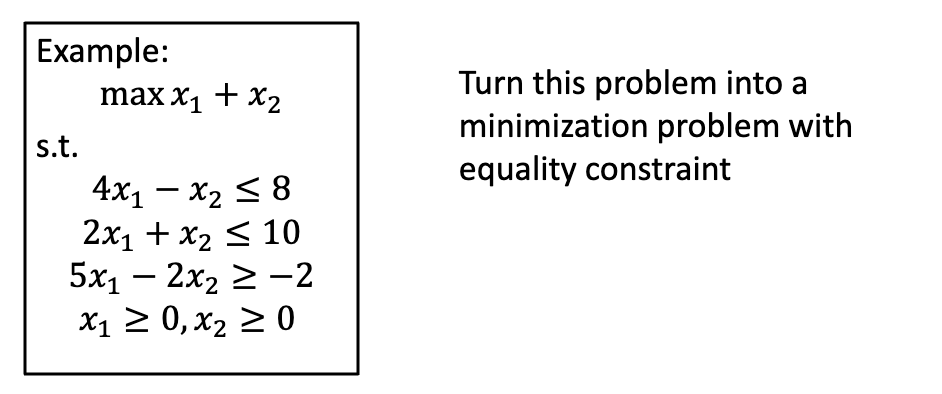
\includegraphics[width=\textwidth]{./images/lp_turn.png}

\begin{verbatim}
min -x_1 - x_2
1. 4x_1 - x_2 + s_1 = 8
2. 2x_1 + x_2 + s_2 = 10
3. 5x_1 - 2x_2 - s_3 = -2
4. x_1, x_2, s_1, s_2, s_3 >= 0
\end{verbatim}

\subsection*{Problem: Maximum Flow}

target: \(\max{f_{sa} + f_{sb} +f_{sc}} \equiv \max{f_{dt} + f_{et}}\)

\subsection*{Linear Regression Problem Reduces to LP}

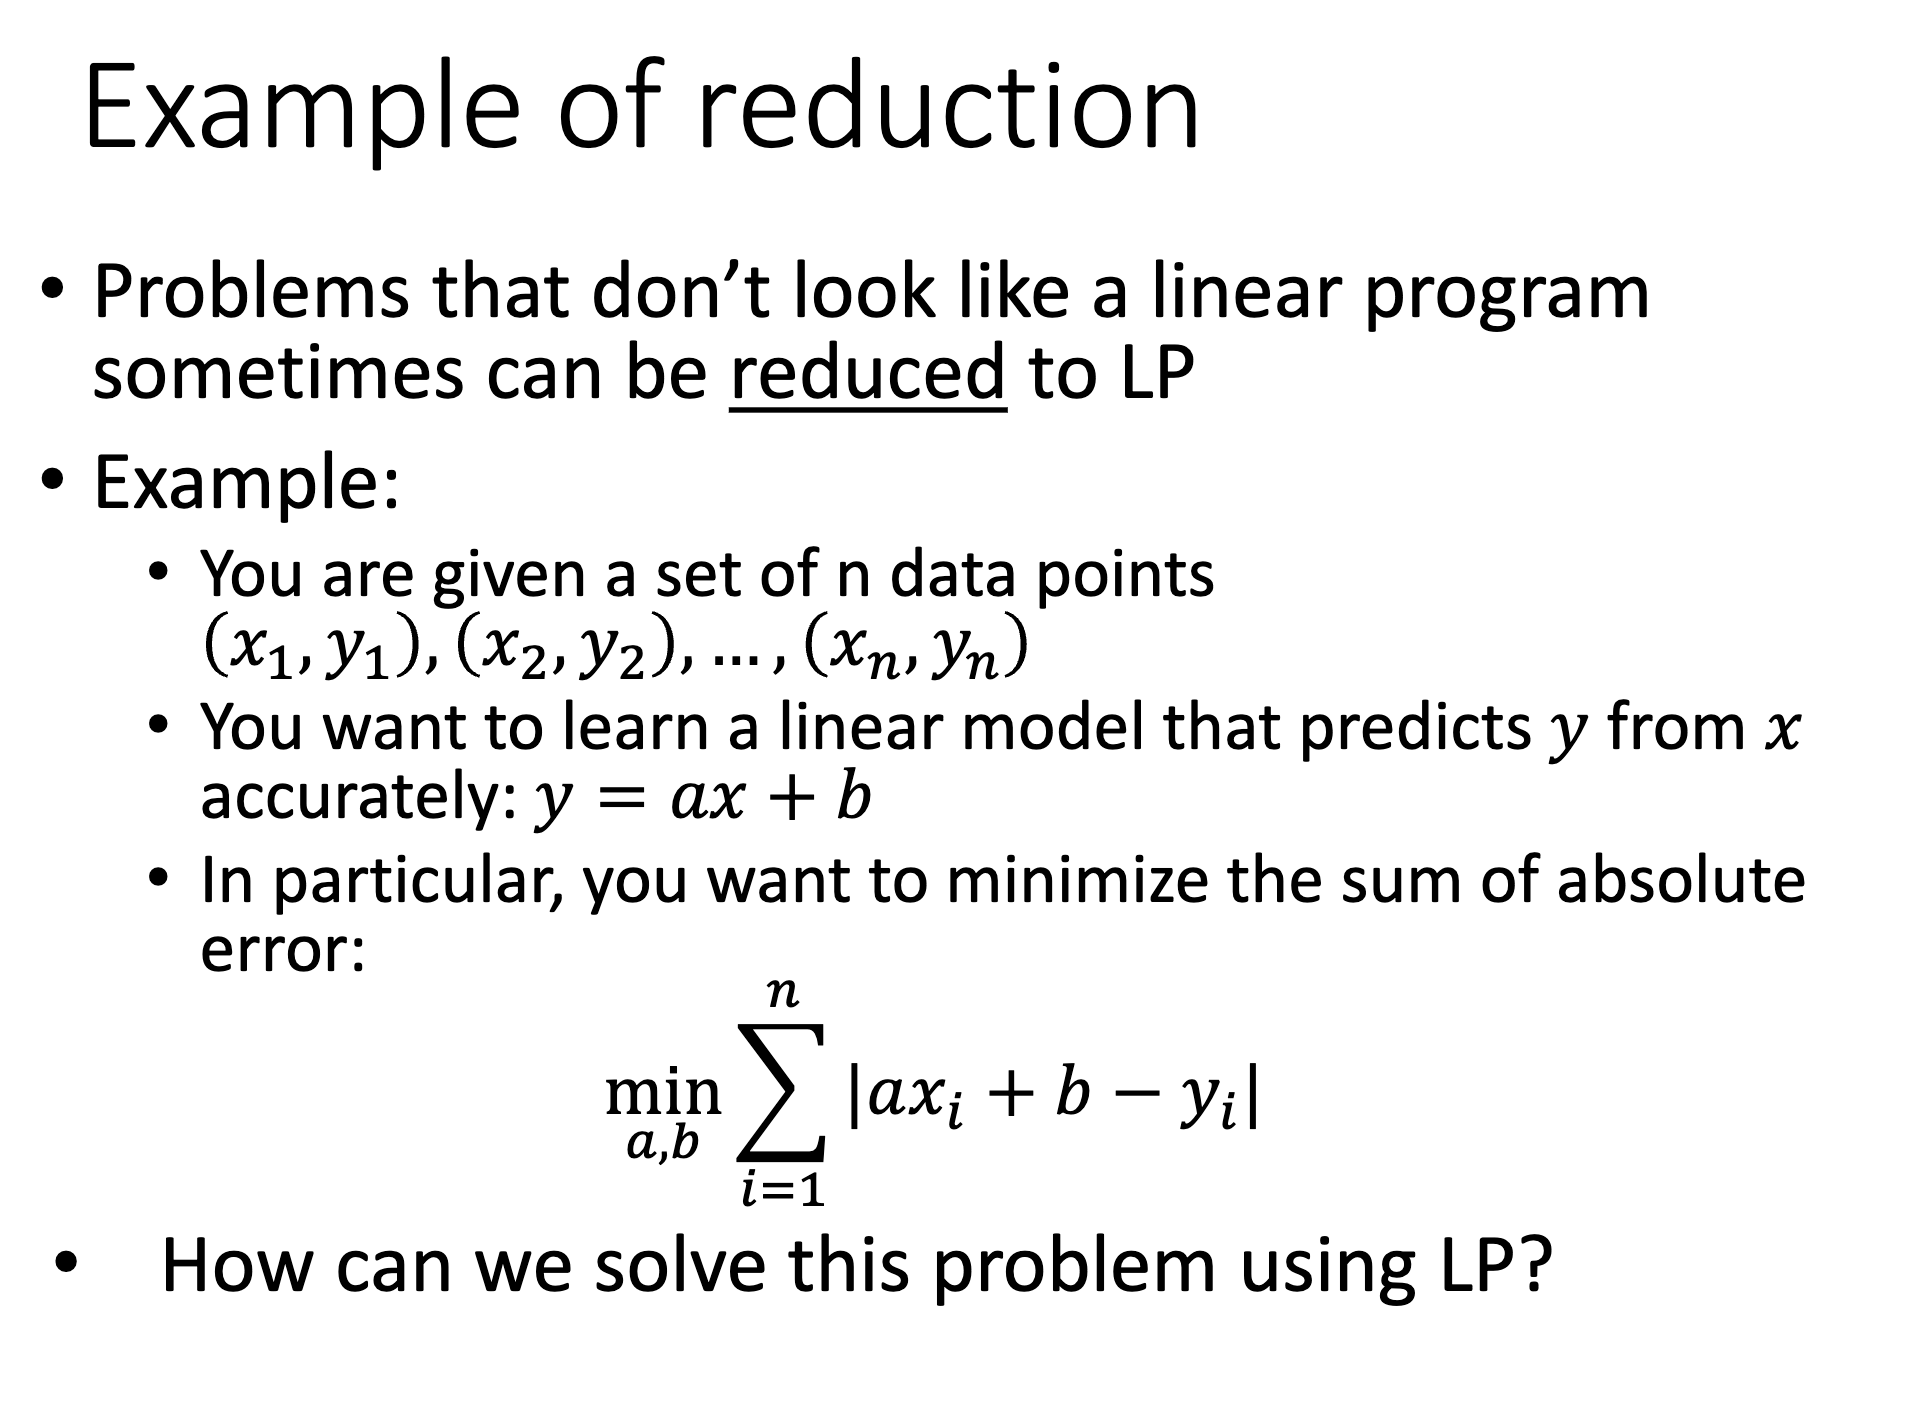
\includegraphics[width=\textwidth]{./images/lr_to_lp.png}

To reduce the given problem to a linear programming (LP) problem, follow these steps:

Given Problem:
We want to minimize the sum of absolute errors:

\[
\min_{a, b} \sum_{i=1}^{n} |a x_i + b - y_i|
\]

Step 1: Introduce Auxiliary Variables

Since absolute values are not directly handled in linear programming, introduce auxiliary variables \( t_i \) for each data point:

\[
t_i \geq |a x_i + b - y_i|, \quad \forall i = 1, 2, \dots, n
\]

Step 2: Reformulate the Absolute Value Constraint

The absolute value constraint can be rewritten as two linear inequalities:

\[
- t_i \leq a x_i + b - y_i \leq t_i, \quad \forall i = 1, 2, \dots, n
\]

Step 3: Formulate the LP Problem

The objective function can now be rewritten as:

\[
\min_{a, b, t_1, t_2, \dots, t_n} \sum_{i=1}^{n} t_i
\]

subject to the constraints:

\[
a x_i + b - y_i \leq t_i, \quad \forall i
\]
\[
a x_i + b - y_i \geq -t_i, \quad \forall i
\]
\[
t_i \geq 0, \quad \forall i
\]

This formulation is now a linear program since the objective function and constraints are all linear.

Conclusion:

By introducing auxiliary variables \( t_i \), the problem is transformed into a standard LP problem. This LP can be solved using simplex or interior-point methods to find the best-fitting line \( y = ax + b \) that minimizes the sum of absolute errors.

\section*{Reduction}



\subsection*{Satisfiability}

Literal: $x_i$ or $\neg x_i$

Clause: A disjunction of clauses $c_j = x_1 \lor x_2 \lor \neg x_3$

CNF $\phi$: A Boolean formula that is a conjunction of clauses \(\phi = c_1 \land c_2 \land c_3 \land c_4\)

\textbf{SAT}: Given a CNF formula $\phi$, does it have a satisfying truth assignment?

\remark{Satisfying truth assignment: assign true/false to each variable such that the entire formula evaluates to true.}

\subsection*{3-SAT to Independent Set}

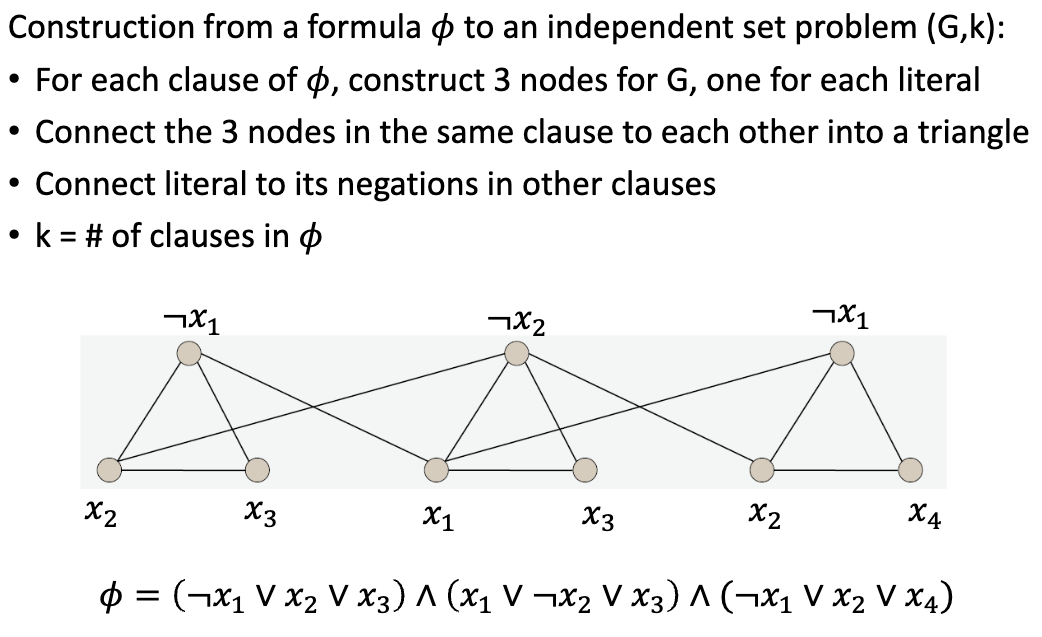
\includegraphics[width=\textwidth]{./images/3sat_reduce_to_is.png}

\subsection*{SAT reduces to 3-SAT}

case where $k<3$

\[k = 2, (l_1 \lor l_2) \Rightarrow (l_1 \lor l_2 \lor x) \land (l_1 \lor l_2 \lor \neg x)\]
\[k = 1, (l_1) \Rightarrow (l_1 \lor x \lor y) \land (l_1 \lor l_2 \lor \neg x)\]

case where $ k>3$

\[ \Rightarrow (l_1 \lor l_2 \lor x_1) \land (\neg x \lor l_3 \lor x_2) \land (\neg x_2 \lor l_4 \lor x_3)\dots\]

if orignally is not satisfiable, new contruct is not satisfiable.

if $l_3 == T$ (statement is satisfiable), just set all free variables after $l_3$ to $F$ and all free variables before $l_3$ to $T$.

\subsection*{3-SAT reduces to Vertex Cover}

3-SAT: A set of clauses, each with exactly 3 literals. Identify whether there exists variables that can be set to true or false such that all clauses are satisfied.

Vertex Cover: Given graph $G$ and integer $k$, does there exist a set of vertices $V'$ such that $|V'| \leq k$ that covers all edges in $G$? 

\section*{Computational Complexity}

\subsection*{Clique}

Certificate: A set of vertices $S \subseteq V$ 

Verification: Check if $|S| = k$ and that every pair of vertices in $S$ is connected by an edge in $E$.

Reduction: $IS \leq_p Clique$

$G = (V, E) \Rightarrow G' = (V, E')$

$E'$ is inverse of $E$.

\subsection*{Hamiltonian Cycle}

Input: A undirected graph $G = (V, E)$

Question: Does there exist a cycle in $G$ that visits each vertex exactly once?

Certificate: A candidate cycle $C$ in $G$

Verification: Check if $C$ is a cycle in $G$ and that it visits each vertex exactly once.

\subsection*{Hamiltonian Cycle-2}



\end{document}